\documentclass[a4paper]{article}
\usepackage{amsmath, amsfonts, amssymb, amsthm}
\usepackage{booktabs}
\usepackage{color}
\usepackage{comment}
\usepackage{enumitem}
\usepackage[top=2cm,bottom=2cm,left=3cm,right=3cm]{geometry}
\usepackage{graphicx}
\usepackage{hyperref}
\usepackage{listings}
\usepackage{tikz}
\usepackage{url}
\usepackage{xspace}
\usepackage{biblatex} % Added for citations
\addbibresource{citations.bib} % Path to your citations.bib file

%%% TIKZ
\usetikzlibrary{calc}
\usetikzlibrary{decorations}
\usetikzlibrary{positioning}
\usetikzlibrary{shapes}

%%% STYLE
\renewcommand{\familydefault}{\sfdefault}
\setlength\parindent{0pt}

%%% ENVIRONMENTS

% Question environment
\newtheoremstyle{que}% name
  {}% Space above, empty = `usual value'
  {}% Space below
  {}% Body font
  {}% Indent amount (empty = no indent, \parindent = para indent)
  {\bfseries}% Thm head font
  {}% Punctuation after thm head
  {\newline}% Space after thm head: \newline = linebreak
  {\thmname{#1}\thmnumber{ #2}:\thmnote{ #3}\vspace{\medskipamount}}% Thm head spec
\theoremstyle{que}
\newtheorem{question}{Question}

%%% MACROS

% Use to fix offset if an environment starts with an enumerate
\newcommand{\fixoffset}{\mbox{}\vspace*{-\bigskipamount}\vspace*{-\medskipamount}}
\newcommand{\eg}{{\em e.g.}\xspace}
\newcommand{\ie}{{\em i.e.}\xspace}
\mathchardef\mhyphen="2D
\newcommand\points[1]{%
\ifnum1<0#1\relax%
    {\bf \small [#1~marks]}%
  \else%
    {\bf \small [#1~mark]}%
  \fi%
}%

\newcommand{\module}{COMP0143: Cryptocurrencies}
\newcommand{\university}{University College London}
\newcommand{\assessment}{Coursework}
\newcommand{\releaseDate}{November 8, 2024}
\newcommand{\dueDate}{December 11, 2024 at 16:00 UK time}
\newcommand{\feedbackDate}{TBD}
\newcommand{\weight}{40\%}
\newcommand{\pointsTotal}{100 marks}

\begin{document}

\title{\module\\[0.25cm]\assessment}
\author{\university}
\date{Released: \releaseDate\\[0.25cm]Due: \dueDate}
\maketitle

\newpage

%%%%%%%%%%%%%%%%%%%%%%%%%%%%%%%%%%%%%%%%%%%%%%%%%

\begin{question}[\points{25}]
  \fixoffset
  \begin{enumerate}[label=(\alph*)]
    \item 
    \item[(i)] To compute \( C \), we first hash our leaves, the elements of \( S \), to get \( H_1, \ldots, H_9 \). We can then compute the internal nodes \( H_{10}, H_{11}, H_{12} \) as follows:
\[
H_{10} = \text{H}(H_1 || H_2 || H_3)
\]
\[
H_{11} = \text{H}(H_4 || H_5 || H_6)
\]
\[
H_{12} = \text{H}(H_7 || H_8 || H_9)
\]
Finally, \( C \) can be calculated as:
\[
C = H_{13} = \text{H}(H_{10} || H_{11} || H_{12})
\]
A figure \ref{fig:merkle_tree} shows the full Merkle Tree.
\begin{figure}[h!]
    \centering
    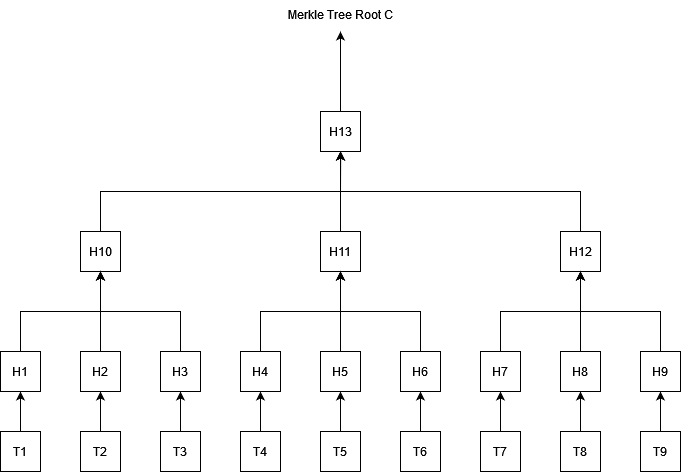
\includegraphics[width=0.5\textwidth]{Merkle Tree example.drawio.png} % Adjust the width as needed
    \caption{Merkle Tree Structure}
    \label{fig:merkle_tree}
To prove \( t_4 \) is in \( S \) we can compute the Merkle Proof as follows:
\[
C = \text{H}(H_{10}||\text{H}(\text{H}(t_4)||H_5||H_6)||H_{12})
\]

\end{figure}
    \item[(ii)] Calculating the Merkle Proof Length \(l\) to show \(t_i\) is in \(S\) is the same as finding height of the tree. From Merkle root to the hashed leaves the number of nodes increases by a multiple of \(m\) so we can calculate the length as \[m^{l-1} = n \rightarrow \log_m n = l - 1\] As \(n\) may not be a multiple of \(m\) we need to take the ceiling of this value and account for the extra hash on input set here shown using \(l-1\). \[ l = \left\lceil \log_m n \right\rceil + 1\]
    \item[(iii)] To minimize the length of the Merkle Proof for a Binary and Ternary Tree we can model the lengths respectively as \[ l = \left\lceil \log_2 n \right\rceil + 1\] and \[ l = \left\lceil \log_3 n \right\rceil + 1\]
    Taking values of n we can compare to see how the functions act for large values shown in table \ref{table:two_column_blank} we can see that Ternary Merkle Trees produce smaller Merkle Proofs.
    \begin{table}[h!]
    \centering
    \begin{tabular}{|c|c|c|}
    \hline
    \textbf{N} & \textbf{Binary Merkle Proof Length} & \textbf{Tenary Merkle Proof Length} \\ 
    \hline
             1000 &  11 &   8   \\ 
    \hline
                  10,000  &  15 &    10            \\ 
    \hline
                100,000     & 18  &      12          \\ 
    \hline
               1,000,000      &  21  &       14        \\ 
    \hline
    \end{tabular}
    \caption{Comparison of length of Merkle Proof for Binary and Tenary trees}
    \label{table:two_column_blank}
    \end{table}
    
    \item Merkle Root hashes are included within the blocks within bitcoin as it provides a logarithmic method to check if a transactions is included in a block shown in previous question. This is more efficient than the linear method of checking each transaction in the full list individually. The impact of not including this would be a decrease in the efficiency of the network as more computation would need to take place to verify inclusion of transactions and each node would need to download the full list of transactions increasing storage., 
    
    \item
    \item[(i)] The privacy coin chosen for this question is Secret Coin \cite{secret_network_graypaper} this was chosen as it uses a unique concept of secret contracts as smart contracts which allows programmable privacy. The aim of the coin is to keep the functionality of the contracts secret while allowing transaction outcome and validity through public ledgers. This is achieved through the use of Trusted Execution Environment(TEE) this ensures that the data is kept , processed and protected in a trusted environment. Encryption functions such as HKDF-SHA256 and HMAC-SHA256 are used to secure contract states by use of unforgable contract keys derived from the signers ID and functions can be used to alter the state of the contract. Zero knowledge proofs are used to validate contract execution which protects sensitive data. SCRT tokens are used as the currency and help provide governance through proof of stake. \cite{secret_foundation_docs}
    
    \item[(ii)] In theory mechanisms such as TEE within secret coin ensure privacy by protecting sensitive data within secret contracts. The network also uses encryption methods to maintain integrity , proof of stake and public ledger helps ensure validity within the system. However in practice some of the mechanisms are vulnerable. The greypaper \cite{secret_network_graypaper} states some method of attack including methods to deanonymise users and circumvent validity showing these are known to the developers. Research on other coins using TEE have found that it is susceptible to side channel attacks and loss of data through TEE crashes \cite{lind2017teechain}. A strength of the TEE is encrypted staking transactions which allows proof of stake without potential to link user identity. The use of encryption methods further helps achieve privacy goals by adding an extra layer of protection to transactions. This is effective for current cryptographic standards but through expansion of network infrastructure or future developments in cryptography , such as quantum cryptography \cite{pirandola2020advances} , could weaken the effectiveness of the privacy.
    
    \item[(iii)]
    Some engineering design choice that could help achieve this goal are alternative consensus mechanism. A paper from 2019 highlights some alternative consensus methods for privacy such as Hyperledger \cite{pahlajani2019survey}. As a method to achieve purely privacy this could be effective but could come at a trade off for reduction scalability. One major restriction of secret coin is the use of Intel-SGX for TEE alternative hardware implementations could improve privacy by providing a more distributed attack surface preventing attackers from targeting specific hardware. A non-engineering design choice that could be added is penalties for privacy breaches. Methods such as penalizing validators who do not protect anonymity of transactions could have stashed tokens removed.
    These are a few design choices that could improve the privacy and anonymity of the secret coin network.
  \end{enumerate}
\end{question}

\newpage

%%%%%%%%%%%%%%%%%%%%%%%%%%%%%%%%%%%%%%%%%%%%%%%%%

\begin{question}[\points{25}]
  \fixoffset
  \begin{enumerate}[label=(\alph*)]
    \item When two miners discover the same block simultaneously both with broadcast their blocks along the network. Other miners will start mining a new block on the chain the received first. After some time has passed one of these chains will grow longer than the other allowing the network to reach consensus on which block is valid resulting in the permanent inclusion in the blockchain. Transactions from the block not accepted are added back into the pool to be used for future blocks. \cite{nakamoto2008bitcoin}
    \item 
    \item Miners can attempt to boycott a misbehaving miner by excluding their mined blocks from the blockchain. These blocks will not be included within the consensus. There are methods the offending miner could circumvent this. The first being having more processing power allowing them to create longer chains which would then be accepted as valid chains. Another could be even if a certain group decides to boycott one miner they blocks could still make it to other miners within the network resulting in the misbehaving miner still participating in the creation of the blockchain. Overall , a miner can boycott a misbehaving minor but this could have varying levels of effectiveness.
    \item 
    \item[(i)] If a miner could put whatever timestamp they wanted within a block they could manipulate Bitcoin's difficulty adjustment algorithm to boost their rewards. An example of such attack would be by manipulating the first and last timestamp within a batch of 2016 blocks to be longer than two weeks, as this is the time frame used to adjust the difficulty. A longer time frame would lower the difficulty allowing for blocks to be mined quicker and therefore increase the rewards gained. However as Bitcoin restricts timestamps this isn't possible.
    \item[(ii)] When a block is produced two timestamps are used the first being the timestamp in the block header by the miner and the second being the actual time the block was produced. Bitcoin uses two rules to ensure the miner timestamp stays inline with policies. The first being that the timestamp is only valid if it is greater than the median of the previous 11 blocks. The second is that the timestamp cannot be greater than two hours in the future relative to the median timestamp of all nodes connected to the miner. \cite{bitcoinwiki_block_timestamp} \cite{bitmex_block_timestamp}
    \item[(iii)] The first rule of ensuring that the block timestamp is greater than the median of the previous 11 blocks helps mitigate attacks by ensuring that time continues to move forward. This prevents attackers from manipulating the blockchains perceived time to be earlier than it actually is resulting in the increase of the block difficulty. The second rule ensures that block time don't get too far ahead limiting them within a two hour window of the actual time. This prevents attackers from attempting to lower the block difficulty. It is still possible to move time forward two hours however this is equivalent to block production rate of 9 minutes and 54 seconds \cite{bitmex_block_timestamp} which has a limited effect on block difficulty.
  \end{enumerate}
\end{question}

\newpage

%%%%%%%%%%%%%%%%%%%%%%%%%%%%%%%%%%%%%%%%%%%%%%%%%

\begin{question}[\points{30}]
  \fixoffset
  \begin{enumerate}[label=(\alph*)]
    \item...
    \item ...
  \end{enumerate}
\end{question}

\newpage

%%%%%%%%%%%%%%%%%%%%%%%%%%%%%%%%%%%%%%%%%%%%%%%%%

\begin{question}[\points{20}]
  As your solution, please submit the completed {\tt TicTacToe.sol} file.
\end{question}

\newpage
% Print the bibliography at the end
\printbibliography

\end{document}
